\documentclass{article}

\usepackage[main=english,vietnamese]{babel}
\usepackage[T1]{fontenc}
\usepackage[utf8]{inputenc}
\usepackage[sexy]{evan}
\usepackage{matchsticks}
\usepackage{wrapfig}
\usepackage{listings}

\newtheorem{hint}{Hint}

\title{The Induction Principle for Beginners - Part I}
\author{Nghia Doan}
\date{\today}

\begin{document}

\maketitle

\begin{definition*}[Induction Principle]
    \label{definition:induction-principle}
    Let $a$ be an integer, and let $P(n)$ be a statement (or proposition) about $n$ for each integer $n \ge a$.
    The \textbf{principle of induction} is a way of proving that $P(n)$ is true for all integers $n \ge a$ in two steps:
    \begin{enumerate}[topsep=0pt, partopsep=0pt, itemsep=0pt]
        \ii \textit{The Base case}: Prove that $P(a)$ is true.
        \ii \textit{The Inductive step}: Assume that $P(k)$ is true for some integer $k \ge a$,
        and use this to prove that $P(k+1)$ is true.
    \end{enumerate}
    Then we may conclude that $P(n)$ is true for all integers $n \ge a$.
\end{definition*}

Our reasoning with the wave of falling dominoes shows that an inductive step is but a shortened form of the chain of theorems
shown in the figure below;
\[
    P(1) \Rightarrow P(2) \Rightarrow P(3) \Rightarrow \cdots \Rightarrow P(k) \Rightarrow P(k+1) \Rightarrow \cdots
\]

We will call theorems in this chain \textit{steps}, and the process of their successive proof \textit{the process of induction}.
This process can be visually represented as a wave of proofs, running from statement to statement along a chain of theorems.

Below is how you can visualize the wave of proofs.

\begin{center}
    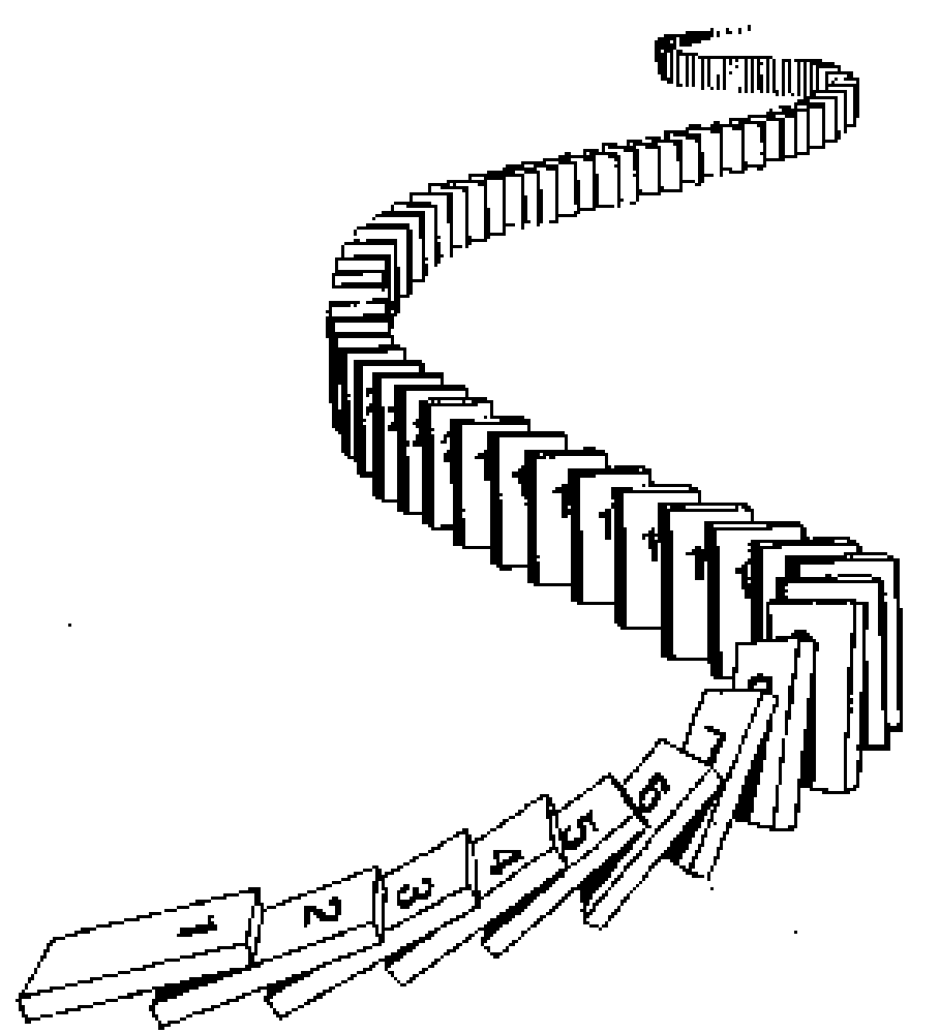
\includegraphics[width=6cm]{./png/cropped-cropped-domino1.png}
\end{center}

The domino effect is the chain reaction consisting of a row of falling dominoes.
The dominoes are vertical and close enough to one another.
One pushes the first domino of the row, and this falls onto the second domino, which falls onto the third domino and so on.
In the end an infinitely long row has fallen!

\newpage

\begin{example}[Example One]
    Show that for all $n \ge 2,$
    \[
        1 \cdot 2 + 2 \cdot 3 + \cdots + (n -1) \cdot n = \frac{(n-1)n(n+1)}{3} \qquad (*)
    \]
\end{example}

\begin{soln}
    Our hypothesis is the given statement, denoted by (*).

    For the base case $n=2,$ $1 \cdot 2 = 2 = \frac{1\cdot 2 \cdot 3}{3},$ thus the hypothesis is true.
    
    Now, for the Inductive step, let's assume that the hypothesis is true for $n,$ or
    \[
        1 \cdot 2 + 2 \cdot 3 + \cdots + (n -1) \cdot n = \frac{(n-1)n(n+1)}{3} \quad (*)
    \]

    We shall prove that
    \[
        1 \cdot 2 + 2 \cdot 3 + \cdots + (n -1) \cdot n +  n\cdot (n+1) = \frac{n(n+1)(n+2)}{3} \quad (**)
    \]

    Using the assumption (*) that the hypothesis is true for $n,$ the left side of (**) can be written as
    \[
        \frac{(n-1)n(n+1)}{3} +  n\cdot (n+1) = n(n+1) \left( \frac{n-1}{3} + 1 \right) = \frac{n(n+1)(n+2)}{3}.
    \]
    Thus, the hypothesis is true for $n+1,$ therefore it is true for all $n \ge 2.$
\end{soln}

\begin{example}[Example Two]
    Show that for all $n \ge 2,$
    \[
        \left(1 - \frac{1}{4}\right) \left(1 - \frac{1}{9}\right) \cdots \left(1 - \frac{1}{n^2}\right) = \frac{n+1}{2n} \qquad (*)
    \]
\end{example}

\begin{soln}
    Our hypothesis is the given statement, denoted by (*).

    For the base case $n=2,$ 
    \[
        \left(1 - \frac{1}{4}\right) = \frac{3}{4} = \frac{2+1}{2\cdot 2}, \text{\  thus the hypothesis is true.}
    \]
    
    Now, for the Inductive step, let's assume that the hypothesis is true for $n,$ or
    \[
        \left(1 - \frac{1}{4}\right) \left(1 - \frac{1}{9}\right) \cdots \left(1 - \frac{1}{n^2}\right) = \frac{n+1}{2n} \quad (*)
    \]

    We shall prove that
    \[
        \left(1 - \frac{1}{4}\right) \left(1 - \frac{1}{9}\right) \cdots \left(1 - \frac{1}{(n+1)^2}\right) = \frac{n+2}{2(n+1)} \quad (**)
    \]

    Using the assumption (*) that the hypothesis is true for $n,$ the left side of (**) can be written as
    \[
        \frac{n+1}{2n} \cdot  \left(1 - \frac{1}{(n+1)^2}\right) = \frac{n+1}{2n} \frac{(n+1)^2-1}{(n+1)^2} 
        = \frac{n+1}{2n} \frac{n(n+2)}{(n+1)^2} = \frac{n+2}{2(n+1)}.
    \]
    Thus, the hypothesis is true for $n+1,$ therefore it is true for all $n \ge 2.$
\end{soln}

\newpage

\begin{example}[Example Three]
    Show that for all $n \ge 1,$
    \[
        n^3 + (n+1)^3 + (n+2)^3 \text{\ is divisible by\ } 9 \qquad (*)
    \]
\end{example}

\begin{soln}
    Our hypothesis is the given statement, denoted by (*).

    For the base case $n=1,$ 
    \[
        1^3 + 2^3 + 3^3 = 9 + 27 \text{\ is divisible by\ } 9.
    \]
    
    Now, for the Inductive step, let's assume that the hypothesis is true for $n,$ or
    \[
        n^3 + (n+1)^3 + (n+2)^3 \text{\ is divisible by\ } 9 \quad (*)
    \]

    We shall prove that
    \[
        (n+1)^3 + (n+2)^3 + (n+3)^3 \text{\ is divisible by\ } 9 \quad (**)
    \]

    Using the assumption (*) that the hypothesis is true for $n,$ the left side of (**) can be written as
    \[
        (n+1)^3 + (n+2)^3 + (n+3)^3 = n^3 + (n+1)^3 + (n+2)^3 + (n+3)^3 - n^3.
    \]

    Since
    \[
        \begin{aligned}
            &(n+3)^3 - n^3 = \left( (n+3)-n\right)\left((n+3)^2 + (n+3)n + n^2\right)
            = 3(3n^2+9n+9) \text{\ is divisible by\ } 9.
        \end{aligned}
    \]
    Thus, the hypothesis is true for $n+1,$ therefore it is true for all $n \ge 1.$
\end{soln}

\begin{example}[Example Four]
    Show that for all $n \ge 1,$
    \[
        11^{n+2} + 12^{2n+1} \text{\ is divisible by\ } 133 \qquad (*)
    \]
\end{example}

\begin{soln}
    Our hypothesis is the given statement, denoted by (*).

    For the base case $n=1,$ 
    \[
        11^{3} + 12^{3} = (11+12)(11^2 - 11\cdot 12 + 12^2) = 23 \cdot 133 \text{\ is divisible by\ } 133.
    \]
    
    Now, for the Inductive step, let's assume that the hypothesis is true for $n,$ or
    \[
        11^{n+2} + 12^{2n+1} \text{\ is divisible by\ } 133 \quad (1)
    \]

    We shall prove that
    \[
        11^{n+3} + 12^{2n+3} \text{\ is divisible by\ } 133 \quad (2)
    \]

    Note that 
    \[
        11^{n+3} + 12^{2n+3} - 11(11^{n+2} + 12^{2n+1}) = 12^{2n+1}(12^2 - 11) = 133 \cdot 12^{2n+1} \text{\ is divisible by\ } 133.
    \]
    
    By (1), $11^{n+3} + 12^{2n+3}$ is divisible by 133, so (2) is true, hence the hypothesis is true for all $n \ge 1.$
\end{soln}

\begin{example}[Example Five]
    Show that for all $n \ge 2,$
    \[
        2^n > 1 + n\sqrt{2^{n-1}}.
    \]
\end{example}

\begin{soln}
    Our hypothesis is that for all $n \ge 2,$
    \[
        (2^n - 1)^2 > n^2 2^{n-1}.
    \]

    For the base case $n=2,$ 
    \[
        (2^2 -1) = 3^2  = 9 > 2^2 \cdot 2^1 = 8.
    \]
    
    Now, for the Inductive step, let's assume that the hypothesis is true for $n,$ or
    \[
        (2^n - 1)^2 > n^2 2^{n-1} \quad (1)
    \]

    We shall prove that
    \[
        (2^{n+1} - 1)^2 > (n+1)^2 2^{n} \quad (2)
    \]

    By the assumption (1),
    \[
        (2^{n+1} - 1)^2 = (2(2^n)-1)^2 = 4(2^n-1)^2 + 4(2^n) + 3 
        > 4 n^2 2^{n-1} + 4 2^n + 3 
    \]
    
    Thus we need to show that
    \[
        4 n^2 2^{n-1} + 4 2^n + 3 > (n+1)^2 2^{n} = n^2 2^{n} + (2n)2^n + 2^n
        \Leftrightarrow n^2 2^{n} + 3 (2^n) + 3 > (2n)2^n
    \]
    Since $n^2 > 2n,$ so the last inequality is true.
    
    Thus (2) is true for $n+1,$ therefore the hypothesis is true for all $n \ge 2.$
\end{soln}

\end{document}